% JKAIA 2026 (2026 한국인공지능학회 추계학술대회) -- General (Poster) track, paper A
% Template: kaia.cls from the official poster-track ZIP (논문제출 안내 page; the ZIP is unchanged since
% 2026-10-01, checked 2026-10-24). Poster rule: a 1--2 page summary with title, authors, affiliations and an
% optional abstract. Review is single-blind, so author names stay in the PDF. Paper in English; the
% EasyChair abstract field is filled in Korean (see ../README.md).
%
% Workflow: main_ko.tex is the Korean WORKING COPY with the same paragraph structure. Edit the Korean text,
% then apply the same edits here paragraph by paragraph. This file is the SUBMISSION.
% Numbers: every number below was recomputed from ../../main/results (2026-10-24); sources in ../README.md.
%
% Build:  tectonic -X compile main.tex   (or pdflatex main; bibtex not needed)
%         python3 build/make_fig.py      (figures/fig_main.pdf from the result CSVs)
%
% Template notes (same as the DriveWAM poster):
%  * kaia.cls \maketitle switches to \twocolumn[...]; the official sample then draws a full-width
%    \fbox{\parbox{\textwidth}{...}}, which cannot break across pages. For a two-page summary we keep one
%    column and draw the same frame with mdframed (page-breakable).
%  * kaia.cls asks for Times via times/mathptmx. Under XeTeX (tectonic) those fonts are not mapped, so we
%    load the system Times New Roman; pdflatex/Overleaf keep the class default.

\documentclass[nouppercase]{kaia}
\usepackage{amsmath}
\usepackage{booktabs}
\usepackage{graphicx}
\usepackage[framemethod=TikZ]{mdframed}
\usepackage{iftex}
\ifXeTeX
  \usepackage{fontspec}
  \setmainfont{Times New Roman}
\fi
\AtBeginDocument{\hypersetup{hidelinks,pdftitle={Planners Exploit Deterministic Error: Dithered Low-Bit World Models},pdfauthor={YongHwi Song, Keon Myung Lee}}}
\graphicspath{{figures/}}

\makeatletter
\renewcommand{\twocolumn}[1][]{#1}   % keep one column; \maketitle's optional argument is still typeset
\makeatother
\mdfsetup{linewidth=0.4pt, linecolor=black, innerleftmargin=7pt, innerrightmargin=7pt,
          innertopmargin=4pt, innerbottommargin=4pt, skipabove=4pt, skipbelow=4pt}
\newcommand{\shiter}{\textsf{sh-iter}}
\newcommand{\dtm}{\textsf{det}}

\title{Planners Exploit Deterministic Error: Dithered Low-Bit World Models}

\author{YongHwi Song}{a}
\author{Keon Myung Lee}{b}
\affiliation{School of Information and Communication Engineering, Chungbuk National University, Korea, thddydgnl1937@gmail.com}{a}
\affiliation{School of Software, Chungbuk National University, Korea, kmlee@cbnu.ac.kr}{b}

\begin{document}

\maketitle
\vspace{-28pt}

\begin{mdframed}

\begin{abstract}
Sampling-based planners query a world model thousands of times per decision, yet low-bit world models fail at planning in ways that bit-width and one-step error do not explain. We show that what matters is the structure of the rounding error rather than its size. Deterministic round-to-nearest leaves an error field that persists across optimizer iterations; in the four tasks where we tested the mechanism, an iterating planner drifts toward the candidates that this error favors. Replacing round-to-nearest with dither (stochastic rounding) shared by all candidates and redrawn at every planner iteration removes most of this drift, at the same bit-width and without training. In internally pre-registered experiments with TD-MPC2 (MPPI, 12 tasks) and DINO-WM (CEM, 3 tasks), deterministic rounding cost up to 100 points of success although its one-step error was no larger than dither's in 29 of 36 affected cells. Dither removed at least half of the damage in all 19 affected Meta-World cells (median 95 percent) and in 4 of 5 \mbox{DINO-WM} cells; in a fused integer kernel (TD-MPC2) the median extra latency was under 10 percent. The fix requires an iterating planner and helps less where little favorable error persists, as on DMC.
\end{abstract}
\begin{keywords}
World models, model-predictive control, quantization, stochastic rounding, robot planning
\end{keywords}

\subsection{Problem Setup}
An MPC planner queries its world model candidates $\times$ iterations $\times$ horizon times per decision: $512\times6\times3$ for the MPPI of TD-MPC2~[1] and $300\times30\times5$ for the CEM of DINO-WM on PushT~[2]. Low-bit inference is the most direct way to cut this cost, but quantized world models break planning in ways that bit-width and offline error do not explain~[3, 4]. We quantize hidden MLP activations (four dynamics and reward layers in TD-MPC2, six predictor blocks in \mbox{DINO-WM}) to $k$ bits on a calibrated uniform grid. Per task, a pre-registered rule picks $k$ on held-out episodes (mainly the largest $k$ at which round-to-nearest, \dtm, loses at least 20 points), and we test $k-1$, $k$ and $k+1$. We ask why \dtm{} hurts planning more than its one-step error suggests, and whether changing only the rounding repairs it.

\subsection{Novelty}
(1) \textit{Measuring exploitation.} The optimizer-exploitation index (OEI), the model-cost error of the executed plan minus that of random first-iteration candidates, splits exactly into a selection term and a drift term. (2) \textit{A two-axis control}: stochastic variants with the same per-entry error that differ only in sharing across candidates and persistence across iterations. (3) \textit{A training-free fix at the same bit-width} (\shiter). We found no prior use of dither or stochastic rounding for low-bit world-model or VLA inference; the closest study~[5] splits candidate-common and action-relative error with oracle repairs, without an iteration axis, a compression error or a deployable fix. These principles (the optimizer's curse~[6], common random numbers, stochastic rounding~[7]) are classical; their application to compressed world models, the two-axis separation and the effect size are new. (4) \textit{Internal pre-registration}: hypotheses, thresholds and code were frozen in timestamped documents before each stage; failed hypotheses are reported (Table~\ref{tab:hyp}).

\subsection{Algorithms}
\textbf{Rounding variants.} With grid step $\Delta$, \dtm{} maps $x$ to $\Delta\,\mathrm{round}(x/\Delta)$; dither maps it to $\Delta\lfloor x/\Delta+u\rfloor$ with $u\sim U[0,1)$, which is unbiased. The stochastic variants differ only in how $u$ is drawn: per candidate (\textsf{ind}); shared by all candidates and redrawn at every forward call, hence fresh at every planner iteration (\shiter, the proposed fix); shared and fixed within a control step (\textsf{sh-step}) or an episode (\textsf{sh-ep}; the two coincide in open-loop CEM). Other planner settings are the official defaults (MPPI: 64 elites; CEM: top 30, 10 iterations on Wall and PointMaze).
\textbf{Exploitation.} With $e(a)$ the cost error of candidate $a$ relative to the unquantized model, $\mathrm{OEI}=e(a_{\mathrm{exec}})-\bar e_{\mathrm{first}}=\text{selection}+\text{drift}$, where the drift is the change of the population-mean error from the first to the last iteration. A negative drift means the planner moved toward candidates that the error favors.
\textbf{Theory.} Fresh unbiased noise has zero expected drift, whereas a persistent field pulls the population to the minimizer of the smoothed model cost (a sample-average-approximation bias). The derived selection and drift terms matched 922k simulated MPPI and CEM runs (fitted slopes 0.92--1.05).

\begin{center}
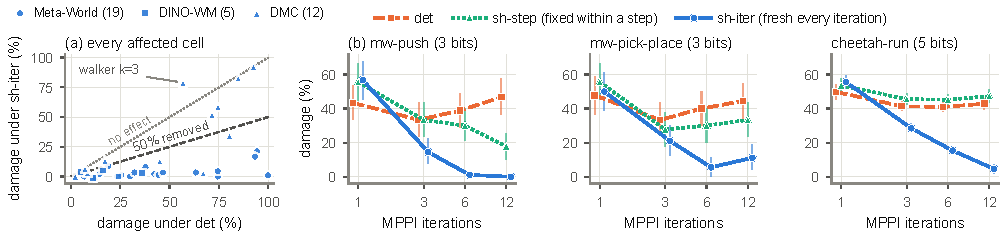
\includegraphics[width=\linewidth]{fig_main.pdf}
\captionof{figure}{(a) Damage under \shiter{} vs.\ \dtm{} in every affected cell (success-rate drop; relative return drop on DMC); below the dashed line \shiter{} removes at least half. (b) Damage vs.\ MPPI iterations (TD-MPC2, 90 paired episodes, 95\% CIs).}
\label{fig:main}
\end{center}

\subsection{Experiments}
\textbf{Setup.} TD-MPC2: official 5M checkpoints (3 seeds), 8 Meta-World tasks (success) and 4 DMC tasks (return), 36 task--bit cells, 90 paired episodes per variant. DINO-WM: official PushT, Wall and PointMaze models, 9 cells, 100 paired episodes. All variants are paired with the unquantized baseline (same seeds and planner noise), and damage $D$ is the drop from it (relative return on DMC). A \dtm{} drop counts as real if it survives per-task Holm correction (paired bootstrap, 95\%); such cells are called affected (31 TD-MPC2 and 5 \mbox{DINO-WM} cells).
\textbf{Phenomenon and fix} (Fig.~\ref{fig:main}a). \dtm{} costs up to 100 points (mw-button-press, 2 bits). In 29 of these 36 affected cells its one-step error is no larger than that of \shiter{} (mw-pick-place, 3 bits: 0.22 vs.\ 0.39, yet 37.8 vs.\ 7.8 points lost). \shiter{} removes at least half of the damage in all 19 affected Meta-World cells (median 95\%) and in 4 of 5 DINO-WM cells, and it is never worse than \dtm{} in any affected Meta-World or \mbox{DINO-WM} cell.
\textbf{Mechanism} (Fig.~\ref{fig:main}b). Under \dtm{} the population-mean error drifts favorably in all four mechanism tasks at their primary bit-widths; \shiter{} keeps at most 24\% of that drift, while persistent dither in TD-MPC2 keeps 70--130\%. The benefit needs iterations: with one iteration \shiter{} is no better than \dtm, but at 12 iterations its damage is 0--11\% while that of \dtm{} stays at 43--47\%. With the elites fixed, exploitation and damage grow with the candidate count (3 of 4 tasks), and the damage of fixed dither shrinks as the number of independent offsets it draws (its table size) grows (5 of 6 tasks).
\textbf{DMC.} The persistent share of \dtm{}'s favorable error (drift over OEI) is 0.33--0.52 on DMC versus 0.54--0.73 on Meta-World, and across the 12 TD-MPC2 tasks it predicts how much \shiter{} helps (Spearman 0.83; a test fixed after stage 1 and run on new seeds). On DMC \shiter{} removes half of the damage in only 5 of 12 cells and is harmful on walker at 3 bits (78.9\% vs.\ 56.9\% of return lost).

\begin{center}
\footnotesize
\setlength{\tabcolsep}{5pt}
\begin{tabular}{@{}p{0.58\linewidth}>{\raggedright\arraybackslash}p{0.38\linewidth}@{}}
\toprule
Hypothesis and pre-registered test & Outcome \\
\midrule
H1: \dtm{} one-step error $\le$ \shiter{} in some affected cell & holds in both families \\
H3a: \shiter{} removes $\ge$50\% in $\ge$75\% of affected cells; none $>$5 pts worse & Meta-World 19/19, DINO-WM 4/5; DMC fails \\
DMC rule (added after stage 1): Spearman of persistent share with gain $\ge0.5$ & holds: 0.83 over 12 tasks \\
H2a$'$ (added after stage 1): \dtm{} drift $<0$, drift ratio \shiter/\dtm{} $<0.5$ & holds: 4/4 tasks (ratio $\le$0.24) \\
H2c: Spearman of $|\mathrm{OEI}_{\dtm}|$ and $D_{\dtm}$ with candidate count $\ge0.8$ & holds: 3/4 tasks \\
H4a: Spearman of fixed-dither damage with table size $\le-0.8$ & holds: 5/6 tasks (three exactly at $-0.8$) \\
H3b: \shiter{} beats \dtm{} on top of the best PTQ in most 3--4-bit cells & TD-MPC2 holds (10/19); DINO-WM fails (1/3) \\
H5: dither latency overhead $\le$10\%; one Pareto-dominating setting & holds weakly (max 6.9\%); no speed-up over fp32 \\
H2a, H2b (original OEI tests); H4b (near-tie density vs.\ sharing gain) & fail (claims narrowed) \\
\bottomrule
\end{tabular}
\captionof{table}{Pre-registered hypotheses and outcomes. Mechanism tasks: mw-push, mw-pick-place, cheetah-run, PushT.}
\label{tab:hyp}
\end{center}

\par\vspace{3pt}\noindent{\scriptsize\textbf{References.}
[1]~N.~Hansen, H.~Su, X.~Wang, TD-MPC2, ICLR, 2024.
[2]~G.~Zhou et al., DINO-WM, arXiv:2411.04983, 2024.
[3]~Z.~Fu et al., An empirical study of world model quantization, arXiv:2602.02110, 2026.
[4]~J.~Xu et al., Predict before you deploy (PreDE), arXiv:2609.19441, 2026.
[5]~R.~Min et al., When low prediction error misleads planning, arXiv:2610.05550, 2026.
[6]~J.~E.~Smith, R.~L.~Winkler, The optimizer's curse, Management Science, 2006.
[7]~S.~Gupta et al., Deep learning with limited numerical precision, ICML, 2015.\par}

\end{mdframed}

\end{document}
